\documentclass[a4paper, 12pt]{article}

\usepackage[spanish]{babel}
\usepackage{hyperref}
\usepackage{amsmath}
\usepackage{listings, xcolor}
\usepackage{caption, subcaption, graphicx}

\definecolor{codegreen}{rgb}{0,0.6,0}
\definecolor{codegray}{rgb}{0.5,0.5,0.5}
\definecolor{codepurple}{rgb}{0.58,0,0.82}
\definecolor{backcolour}{rgb}{0.95,0.95,0.92}
\lstdefinestyle{mystyle}{
    backgroundcolor=\color{backcolour},   
    commentstyle=\color{codegreen},
    keywordstyle=\color{magenta},
    numberstyle=\tiny\color{codegray},
    stringstyle=\color{codepurple},
    basicstyle=\ttfamily\footnotesize,
    breakatwhitespace=false,         
    breaklines=true,                 
    captionpos=b,                    
    keepspaces=true,                 
    numbers=left,                    
    numbersep=5pt,                  
    showspaces=false,                
    showstringspaces=false,
    showtabs=false,                  
    tabsize=2
}

\setlength{\parindent}{0pt}
\setlength{\parskip}{8pt}
\lstset{style=mystyle, language=Python}

\title{\vspace{-3cm}Tarea 2: Filtros de Convolución}
\author{
    Angel de Jesús Maldonado Juárez\\
    Universidad Autónoma de San Luis Potosí\\
    Facultar de Ingeniería - Ing. En Sistemas Inteligentes\\
    \textbf{Materia:} Visión Computacional\\
    \textbf{Prof:} Dr. César Augusto Puente Montejano\\
    \textbf{Autor:} Angel de Jesús Maldonado Juárez
}
\date{\textbf{Fecha de entrega:} lunes 19 de septiembre de 2022}

\begin{document}
\maketitle

\begin{center}
    \rule{\textwidth}{0.5pt}
    \begin{abstract}
        \noindent Los filtros en las imágenes se reducen a operaciones con matrices, y existen varios tipos de filtros, cada uno se caracteriza por aplicar una convolución de forma particular para conseguir un efecto final deseado. En este reporte se describen algunos filtros que maneja la librería OpenCV con Python junto con ejemplos prácticos y con los resultados.
    \end{abstract}
    \rule{\textwidth}{0.5pt}
\end{center}

\section{Bilateral Filter}
Cuando se quiere reducir el ruido de una imagen generalmente se le aplica un filtro de suavizado, sin embargo, la mayoría de estos filtros ocasionan pérdida de información en la imagen y a pesar de que logran reducir el ruido de la imagen, le da un efecto borroso en partes no deseadas como los bordes. El \textbf{filtro bilateral} soluciona este problema utilizando, además del \emph{Suavizado Gausiano}, un \emph{peso tonal} que le da mayor importancia a los píxeles que tengan una intensidad similar al pixel del centro de la máscara del filtro.

\begin{equation}
    g(x) = \frac
    {
        \int_{R} f(y) G(x - y) G^t(f(x) - f(y))\,dy
    }
    {
        \int_{R} G(x - y) G^t(f(x) - f(y))\,dy
    }
\end{equation}

El componente $\int_{R} f(y) G(x - y)\,dy$ representa el \emph{Filtro Gausiano}, el cual depende únicamente de la distancia entre $x$ y $y$, a la función de este filtro se le agrega el peso de la \emph{distancia tonal} el cual es representado por $f(y) - f(x)$.

La función de OpenCV que aplica este filtro es \lstinline{bilateralFilter()}, la cual tiene los siguientes parámetros:

\begin{itemize}
    \item \lstinline{src}: imagen a procesar.
    \item \lstinline{d}: diámetro de los pixeles vecinos al pixel del centro (esto define también el tamaño del \emph{kernel}).
    \item \lstinline{sigmaColor}: indica la influencia del color de los pixeles vecinos, a mayor valor se tendrán en cuenta los pixeles más lejanos y se mostrarán áreas de colores similares.
    \item \lstinline{sigmaSpace}: establece el límite de influencia de los pixeles vecinos al centro, siempre y cuando tengan un color similar.
\end{itemize}

\textbf{Ejemplo (Python)}
\begin{lstlisting}
    import cv2 as cv # importar opencv

    # lee la imagen
    img = cv.imread('../img/dog.jpg')
    # aplica filtro a la imagen
    dst = cv.bilateralFilter(img, d, sigmaColor, sigmaSpace)

    # muestra la imagen
    cv.imshow('Bilateral filter', dst)
\end{lstlisting}

\begin{figure}[!ht]
    \centering
    \begin{subfigure}{0.4\textwidth}
        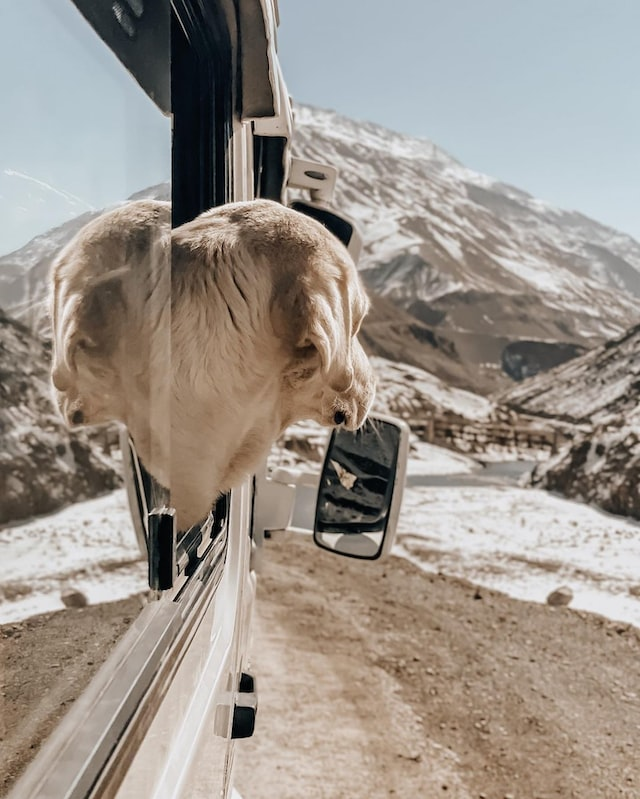
\includegraphics[width=\textwidth]{img/dog.jpg}
        \caption{Imagen original}
    \end{subfigure}
    \begin{subfigure}{0.4\textwidth}
        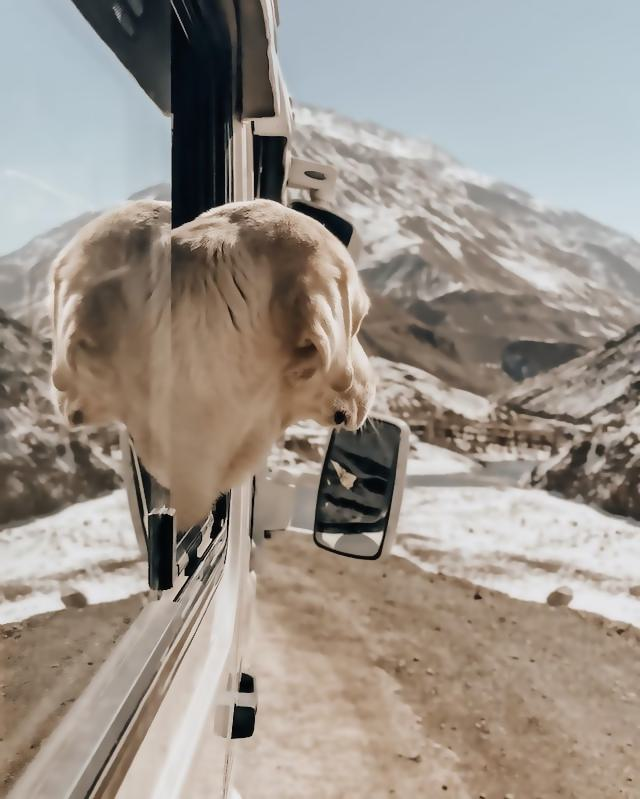
\includegraphics[width=\textwidth]{img/dog-bilateral.jpg}
        \caption{d=9,sigmaColor/Space=75}
    \end{subfigure}
\end{figure}

\section{Blur}
El efecto \emph{blur} o \emph{suavizado} simple en una imagen, también es llamado \emph{box blur}, y su función principal es difuminar todos píxeles de una imagen utilizando el valor promedio de los píxeles más cercanos.

\begin{equation}
    K = \frac{1}{kwidth*kheight}
    *
    \begin{bmatrix}
        1 & 1 & 1 & ... & 1 & 1 \\
        1 & 1 & 1 & ... & 1 & 1 \\
        ...                     \\
        1 & 1 & 1 & ... & 1 & 1 \\
    \end{bmatrix}
\end{equation}

Este \emph{kernel} normaliza las dimensiones de la máscara.

\textbf{Ejemplo (Python)}
\begin{lstlisting}
    import cv2 as cv # importar opencv

    # lee la imagen
    img = cv.imread('../img/dog.jpg')
    # aplica filtro a la imagen
    dst = cv.blur(img, (9,9))

    # muestra la imagen
    cv.imshow('Blur filter', dst)
\end{lstlisting}

\begin{figure}[!ht]
    \centering
    \begin{subfigure}{0.4\textwidth}
        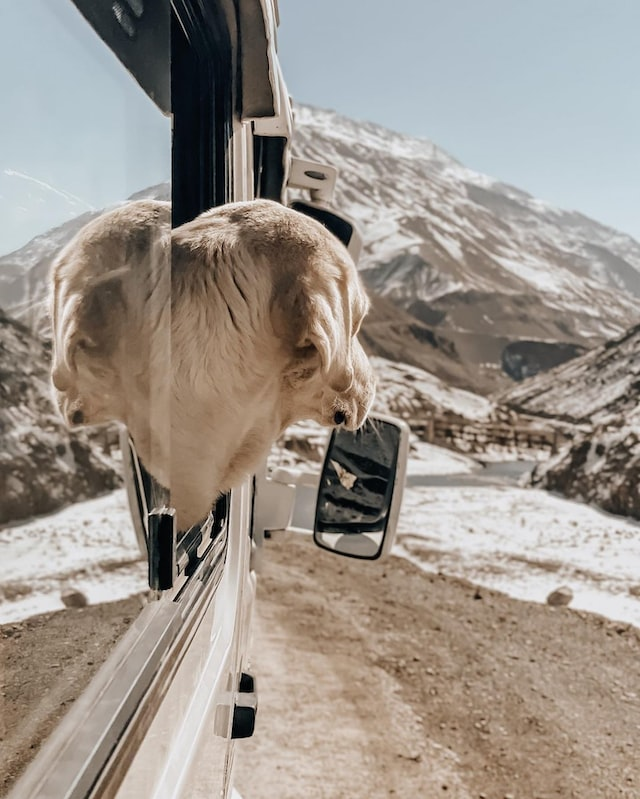
\includegraphics[width=\textwidth]{img/dog.jpg}
        \caption{Imagen original}
    \end{subfigure}
    \begin{subfigure}{0.4\textwidth}
        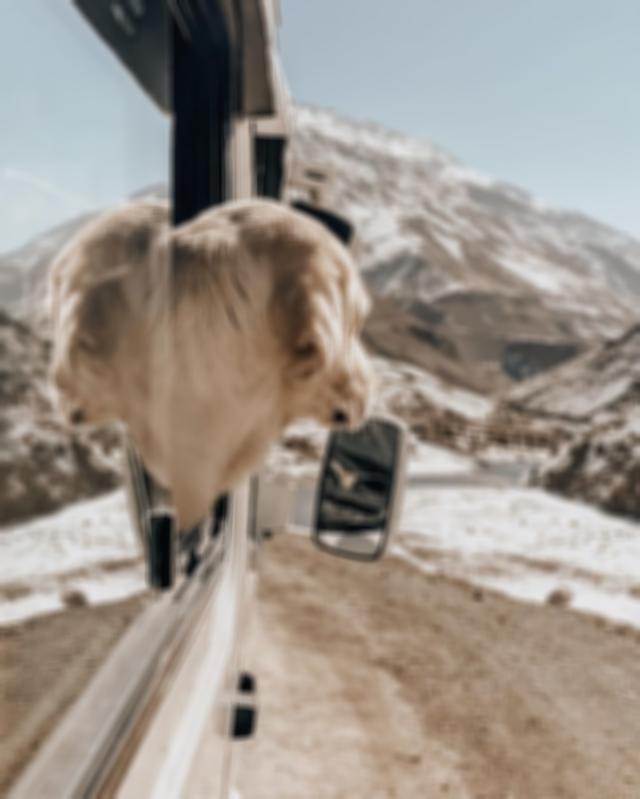
\includegraphics[width=\textwidth]{img/dog-blur.png}
        \caption{ksize=(9,9)}
    \end{subfigure}
\end{figure}

\section{Dilate}
La operación de dilatación consiste en expandir los píxeles de valor máximo en una imagen. El kernel que se utiliza tiene definido un \emph{punto de anchura}, que suele ser el centro del kernel, y cuando se aplica la convolución del kernel a la imagen, se calcula el pixel con mayor valor $(x',y')$ en el kernel y este se incrementa al punto de anchura $(x,y)$:

\begin{equation}
    dst(x,y)=max_{(x',y'):element(x',y')\neq 0}src(x+x',y+y')
\end{equation}

\textbf{Ejemplo (Python)}

\begin{lstlisting}
    import cv2 as cv

    # lee la imagen
    img = cv.imread('../img/dog.jpg')

    # crear el kernel
    kernel = cv.getStructuringElement(cv.MORPH_RECT, (9, 9))

    # aplica filtro a la imagen
    dst = cv.dilate(img, kernel)

    # muestra la imagen
    cv.imshow('Dilate filter', img)
\end{lstlisting}

\begin{figure}[!ht]
    \centering
    \begin{subfigure}{0.4\textwidth}
        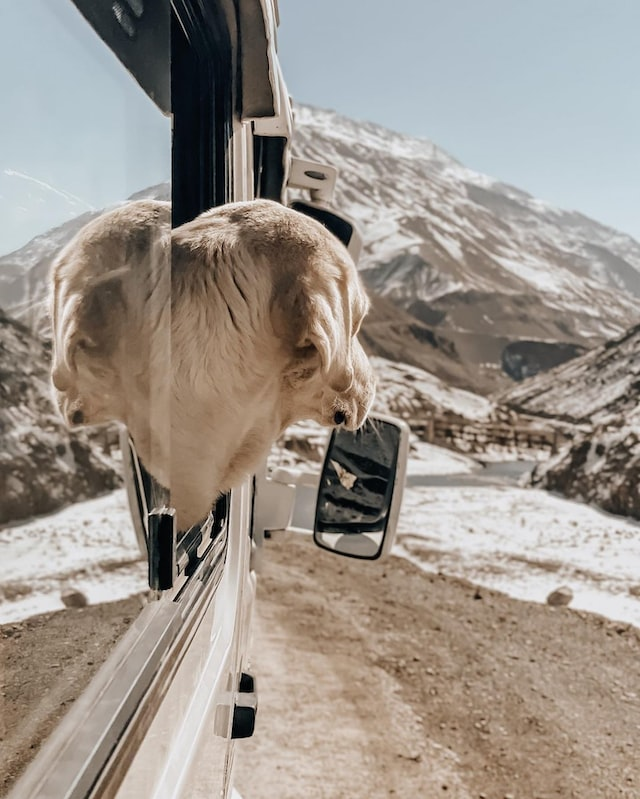
\includegraphics[width=\textwidth]{img/dog.jpg}
        \caption{Imagen original}
    \end{subfigure}
    \begin{subfigure}{0.4\textwidth}
        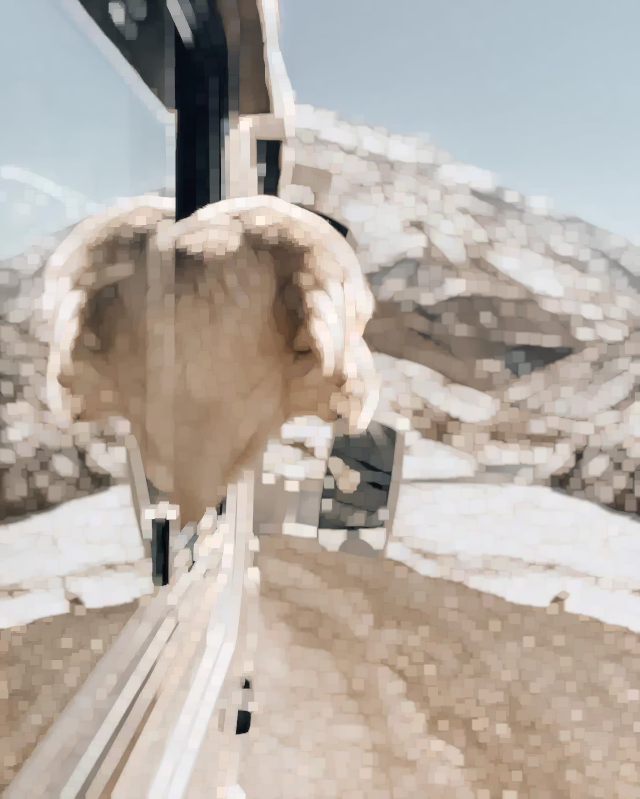
\includegraphics[width=\textwidth]{img/dog-dilate.png}
        \caption{shape=RECT,ksize=(9,9)}
    \end{subfigure}
\end{figure}

\section{Erosion}
Es la operación contraria a la dilatación; con base en el tamaño del kernel, si al aplicar la convolución del kernel a la imagen todos los pixeles al rededor del kernel son $1$ se conservan, de lo contrario el pixel se erosiona (se hace $0$).

\begin{equation}
    dst(x,y)=min_{(x',y'):element(x',y')\neq 0}src(x+x',y+y')
\end{equation}

\textbf{Ejemplo (Python)}
\begin{lstlisting}
    import cv2 as cv

    # lee la imagen
    img = cv.imread('../img/dog.jpg')

    # crear el kernel
    kernel = cv.getStructuringElement(cv.MORPH_RECT, (9, 9))

    # aplica filtro a la imagen
    dst = cv.erode(img, kernel)

    # muestra la imagen
    cv.imshow('Dilate filter', img)
\end{lstlisting}

\begin{figure}[!ht]
    \centering
    \begin{subfigure}{0.4\textwidth}
        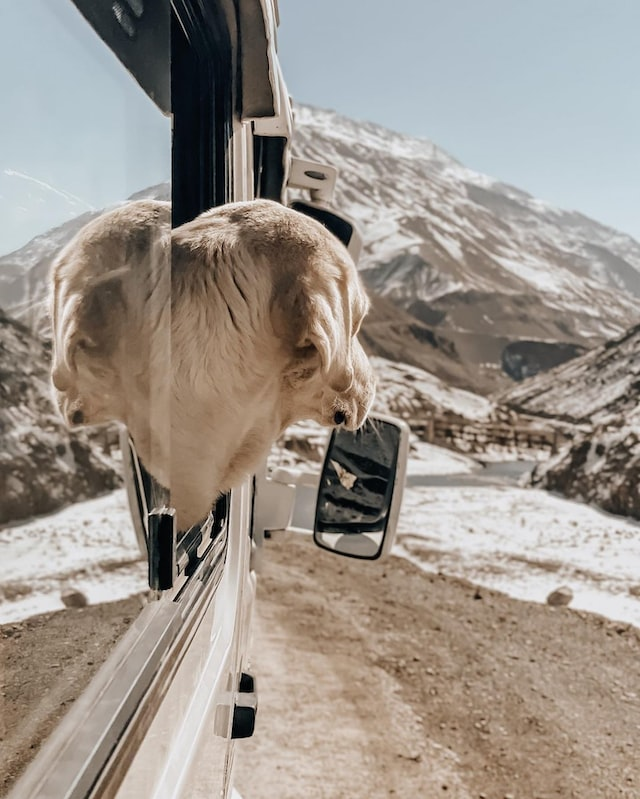
\includegraphics[width=\textwidth]{img/dog.jpg}
        \caption{Imagen original}
    \end{subfigure}
    \begin{subfigure}{0.4\textwidth}
        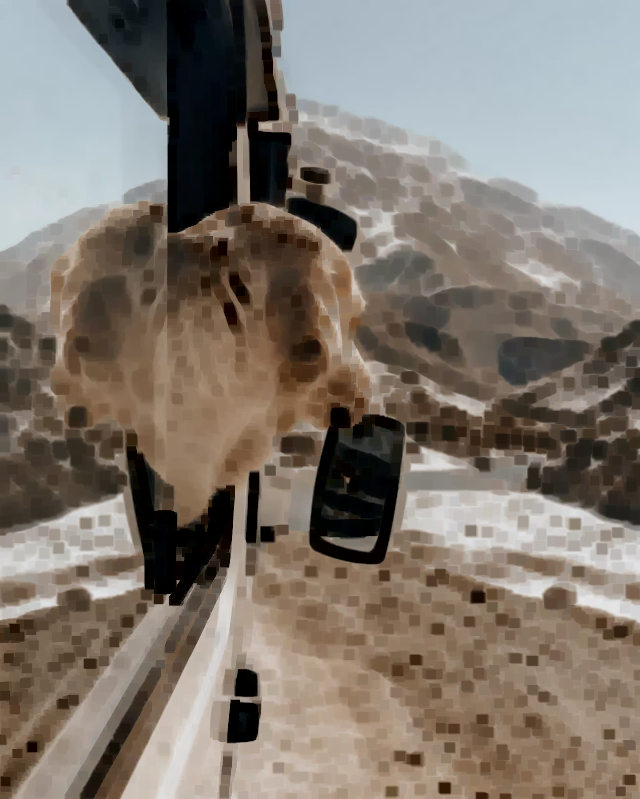
\includegraphics[width=\textwidth]{img/dog-erode.png}
        \caption{shape=RECT,ksize=(9,9)}
    \end{subfigure}
\end{figure}

\section{Gaussian Blur}
Este filtro aplica la \emph{función Gausiana} como método de convolución en la imagen:

\begin{equation}
    g(x,y)=\frac{1}{2\pi \sigma^2}\exp^{-(x^2+y^2)/(2\sigma^2)}
\end{equation}

El argumento $\sigma$ representa la desviación estándar $(x,y)$ de la función Gausiana, este parámetro en la función \lstinline{GaussianBlur()} de de OpenCV lo divide en desviación para $x$ (\lstinline{sigmaX}) y para $y$ (\lstinline{sigmaY}). Mientras mayor sea la desviación, mayor será el efecto de difuminado (\emph{blur}).

\textbf{Ejemplo (Python)}

\begin{lstlisting}
    import cv2 as cv

    # lee la imagen
    img = cv.imread('../img/dog.jpg')

    # aplica filtro a la imagen
    dst = cv.GaussianBlur(img, (9, 9), 12, 12)

    # muestra la imagen
    cv.imshow('Gaussian filter', img)
\end{lstlisting}

\begin{figure}[!ht]
    \centering
    \begin{subfigure}{0.4\textwidth}
        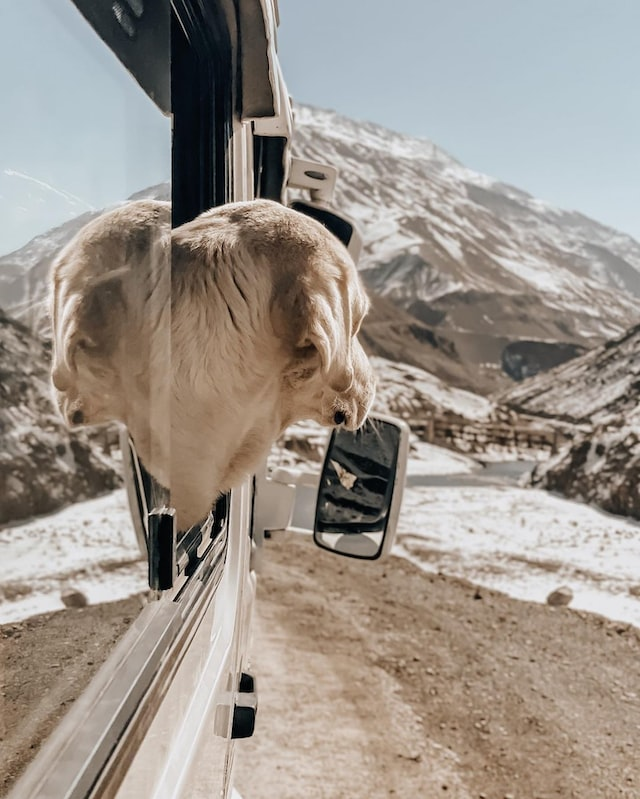
\includegraphics[width=\textwidth]{img/dog.jpg}
        \caption{Imagen original}
    \end{subfigure}
    \begin{subfigure}{0.4\textwidth}
        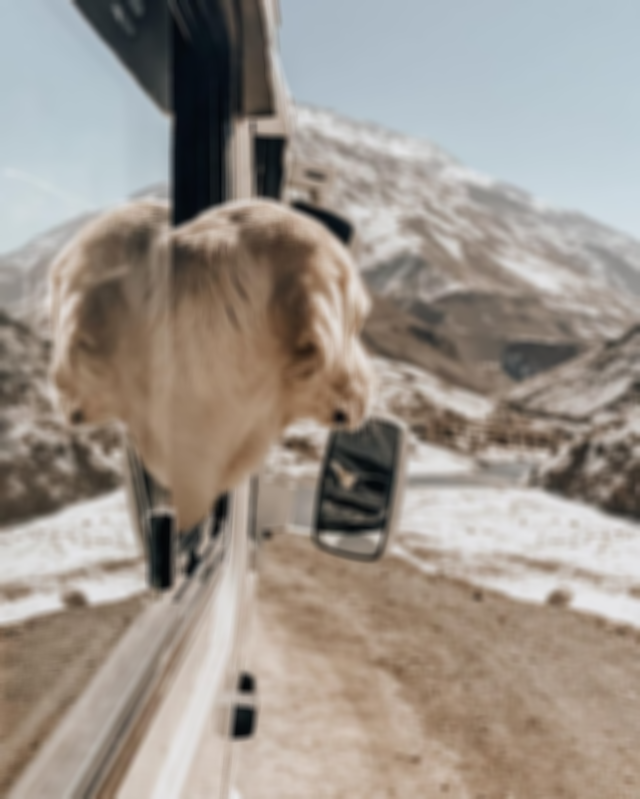
\includegraphics[width=\textwidth]{img/dog-gaussian.png}
        \caption{ksize=(9,9),sigmaX/Y=12}
    \end{subfigure}
\end{figure}

\section{Median Blur}
Mientras que el Filtro Gausiano utiliza el promedio como principal herramienta de convolución, el filtro Median Blur utiliza la mediana de los pixeles al rededor del kernel para reemplazar el pixel central del mismo. Teniendo entonces un único parámetro en la función de OpenCV \lstinline{medianBlur()}: \lstinline{ksize} que es el tamaño del kernel, que también representa la cantidad de pixeles que va a tomar para realizar la convolución.

\textbf{Ejemplo (Python)}

\begin{lstlisting}
    import cv2 as cv

    # lee la imagen
    img = cv.imread('../img/dog.jpg')

    # aplica filtro a la imagen
    dst = cv.medianBlur(img, 9)

    # muestra la imagen
    cv.imshow('Median filter', img)
\end{lstlisting}

\begin{figure}[!ht]
    \centering
    \begin{subfigure}{0.4\textwidth}
        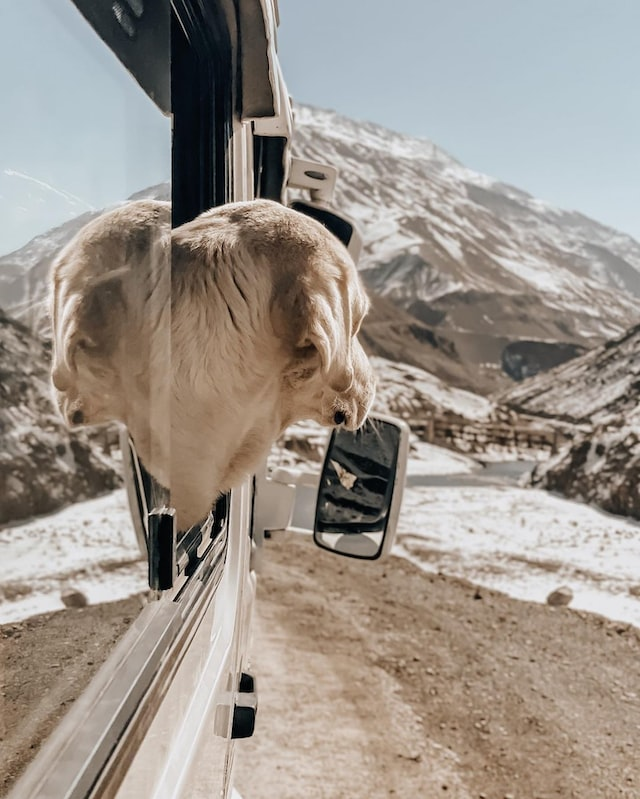
\includegraphics[width=\textwidth]{img/dog.jpg}
        \caption{Imagen original}
    \end{subfigure}
    \begin{subfigure}{0.4\textwidth}
        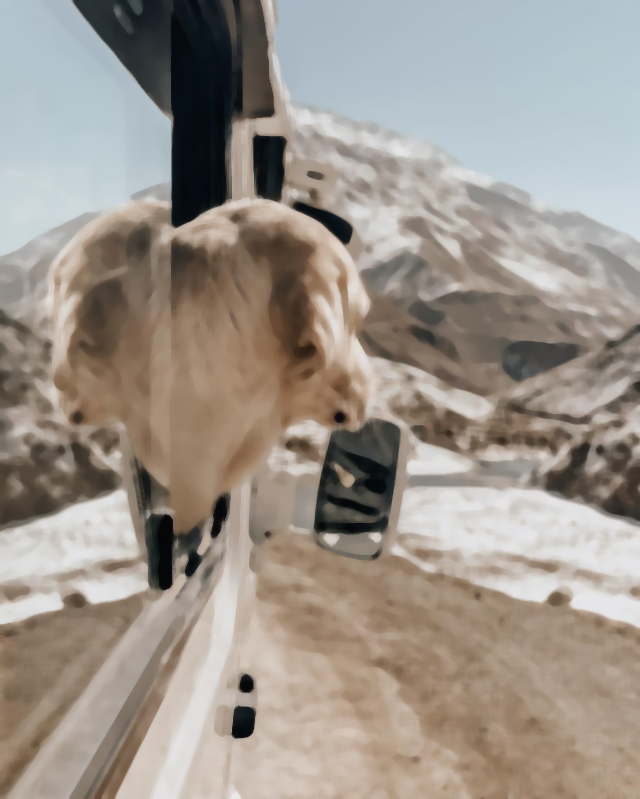
\includegraphics[width=\textwidth]{img/dog-median.png}
        \caption{ksize=9}
    \end{subfigure}
\end{figure}

\section{Spatial Gradient}
Este filtro calcula la derivada de primer orden de una imagen en $x$ y $y$ utilizando el \textbf{operador Sobel}. Este operador utiliza dos kernels de $3x3$ que convolucionan con la imagen para calcular las derivadas, una matriz es para cambios horizontales $G_x$ y otra para los verticales $G_y$:

\begin{equation}
    G_x
    =
    \begin{bmatrix}
        +1 & 0 & -1 \\
        +2 & 0 & -2 \\
        +1 & 0 & -1
    \end{bmatrix}
    *
    A,
    G_y
    =
    \begin{bmatrix}
        +1 & +2 & +1 \\
        0  & 0  & 0  \\
        -1 & -2 & -1 \\
    \end{bmatrix}
\end{equation}

El kernel Sobel puede descomponerse como el producto de un kernel de promedio y un kernel de diferenciación:

\begin{equation}
    G_x
    =
    \begin{bmatrix}
        1 \\
        2 \\
        1
    \end{bmatrix}
    *(
    \begin{bmatrix}
        +1 & 0 & -1
    \end{bmatrix}
    *
    A
    ),
    G_y
    =
    \begin{bmatrix}
        +1 & +2 & +1 \\
        0  & 0  & 0  \\
        -1 & -2 & -1
    \end{bmatrix}
    *
    A
\end{equation}

La función de OpenCV en Python que realiza esta operación de aplicar las derivadas en $x,y$ a la imagen es \lstinline{spatialGradient()}, la cual toma como único parámetro la imagen fuente en formato de blanco y negro, por lo que debe auxiliarse de la función \lstinline{cvtColor()} junto con el enumerable \lstinline{COLOR_BGR2GRAY} para convertir los canales de una imagen a color en blanco y negro. La función \lstinline{spatialGradient} devuelve las matrices resultantes de aplicar la primera derivada a la imagen en $x$ y $y$, por lo que deben de convertirse cada valor de la matriz a su valor absoluto con la función \lstinline{convertScaleAbs()}. Finalmente, para obtener la imagen con el filtro se deben combinar las matrices derivadas, para ello se utiliza la función \lstinline{addWeighted()}, la cual además de combinar las matrices, da la opción de dar mayor peso a cualquiera de las dos matrices, además de agregar brillo con el parámetro \lstinline{gamma}.

\textbf{Ejemplo (Python)}

\begin{lstlisting}
    import cv2 as cv

    # lee la imagen
    img = cv.imread('../img/dog.jpg')
    # convierte la imagen a b&n
    img = cv.cvtColor(img, cv.COLOR_BGR2GRAY)

    # obten las derivadas x,y de la imagen
    dx, dy = cv.spatialGradient(img)
    # convierte al valor absoluto de las matrices derivadas
    abs_grad_x = cv.convertScaleAbs(dx)
    abs_grad_y = cv.convertScaleAbs(dy)

    # suma las matrices dando un peso y brillo final
    dst = cv.addWeighted(abs_grad_x, 0.5, abs_grad_y, 0.5, 0)

    # muestra la imagen final
    cv.imshow('Spatial Gradient', dst)
\end{lstlisting}

\begin{figure}[!ht]
    \centering
    \begin{subfigure}{0.4\textwidth}
        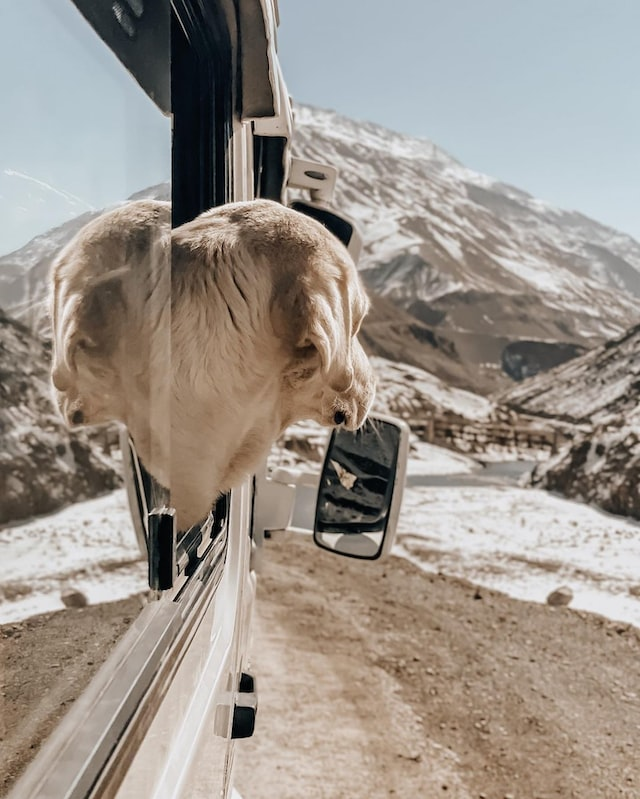
\includegraphics[width=\textwidth]{img/dog.jpg}
        \caption{Imagen original}
    \end{subfigure}
    \begin{subfigure}{0.4\textwidth}
        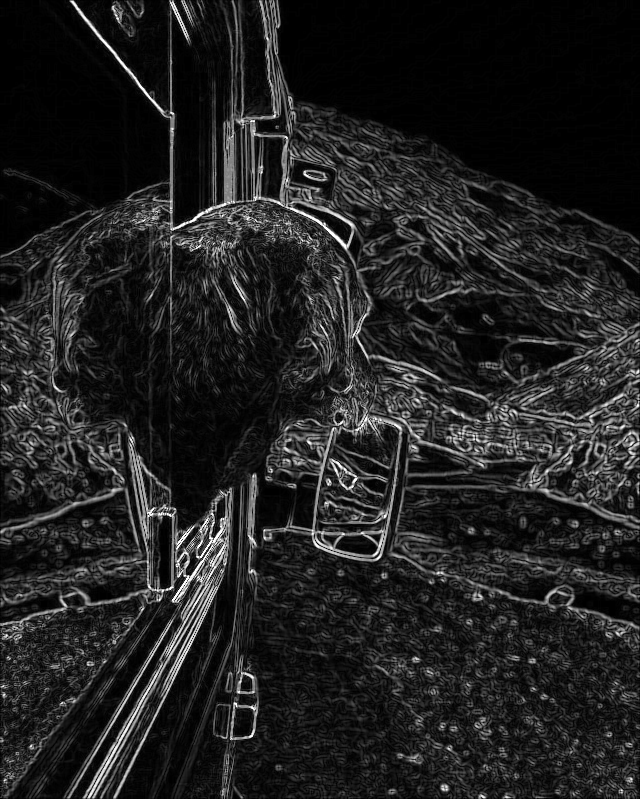
\includegraphics[width=\textwidth]{img/dog-spatial.png}
        \caption{wx/y=0.5,gamma=0}
    \end{subfigure}
\end{figure}

\bibliographystyle{plain}
\bibliography{refs}
\nocite{*}
\end{document}